%%%%%%%%%%%%%%%%%%%%%%% file template.tex %%%%%%%%%%%%%%%%%%%%%%%%%
%
% This is a general template file for the LaTeX package SVJour3
% for Springer journals.          Springer Heidelberg 2010/09/16
%
% Copy it to a new file with a new name and use it as the basis
% for your article. Delete % signs as needed.
%
% This template includes a few options for different layouts and
% content for various journals. Please consult a previous issue of
% your journal as needed.
%
%%%%%%%%%%%%%%%%%%%%%%%%%%%%%%%%%%%%%%%%%%%%%%%%%%%%%%%%%%%%%%%%%%%
%
% First comes an example EPS file -- just ignore it and
% proceed on the \documentclass line
% your LaTeX will extract the file if required
%\begin{filecontents*}{example.eps}
%!PS-Adobe-3.0 EPSF-3.0
%%BoundingBox: 19 19 221 221
%%CreationDate: Mon Sep 29 1997
%%Creator: programmed by hand (JK)
%%EndComments
%gsave
%newpath
%  20 20 moveto
%  20 220 lineto
%  220 220 lineto
%  220 20 lineto
%closepath
%2 setlinewidth
%gsave
%  .4 setgray fill
%grestore
%stroke
%grestore
%\end{filecontents*}
%
\RequirePackage{fix-cm}
\RequirePackage{amsmath}
%
%\documentclass{svjour3}                     % onecolumn (standard format)
%\documentclass[smallcondensed]{svjour3}     % onecolumn (ditto)
%\documentclass[smallextended]{svjour3}       % onecolumn (second format)
\documentclass[twocolumn]{svjour3}          % twocolumn
%
\smartqed  % flush right qed marks, e.g. at end of proof
%
\usepackage{graphicx}
%
\usepackage{mathptmx}      % use Times fonts if available on your TeX system
%
% insert here the call for the packages your document requires
\let\amalg\relax
\usepackage{amssymb,
mathtools,bm,extraipa,mathabx,graphicx,algorithm}
\usepackage{algpseudocode}
\usepackage{url}

%\usepackage{latexsym}
% etc.
%
% please place your own definitions here and don't use \def but
% \newcommand{}{}

\newcommand{\fudge}{\fC}
\newcommand{\cc}{\mathcal{C}}
\newcommand{\dtf}{\textit{\doubletilde{f}}}
\newcommand{\cube}{[0,1]^d}
\newcommand{\rf}{\mathring{f}}
\newcommand{\rnu}{\mathring{\nu}}
\newcommand{\natm}{\naturals_{0,m}}
\newcommand{\wcS}{\widecheck{S}}
\newcommand{\tol}{\text{tol}}
\newcommand{\e}{\text{e}}
%\newcommand{\bvec}[1]{\boldsymbol{#1}}
\newcommand{\vect}[1]{\boldsymbol{\mathbf{#1}}}
\newcommand{\vx}{\vect{x}}
\newcommand{\vI}{\vect{I}}
\newcommand{\vk}{\vect{k}}
\newcommand{\vw}{\vect{w}}
\newcommand{\vz}{\vect{z}}
\newcommand{\vt}{\vect{t}}
\newcommand{\dif}{\mathsf{d}}
\newcommand{\hf}{\hat{f}}
\newcommand{\hS}{\widehat{S}}
\newcommand{\tS}{\widetilde{S}}
\newcommand{\tf}{\tilde{f}}
\newcommand{\fC}{\mathfrak{C}}
\newcommand{\homega}{\widehat{\omega}}
\newcommand{\wcomega}{\mathring{\omega}}
\newcommand{\vzero}{\vect{0}}
\newcommand{\integers}{\mathbb{Z}}
\newcommand{\naturals}{\mathbb{N}}
\newcommand{\ip}[3][{}]{\ensuremath{\left \langle #2, #3 \right \rangle_{#1}}}
\newcommand\iid{\stackrel{{\rm iid}}{\sim}}

\makeatletter
\newcommand{\ov}[1]{
  \m@th\overline{\mbox{#1}\raisebox{2mm}{}}
}
\newcommand{\absolute}[1]{\left\lvert#1\right\rvert}
\let\oldemptyset\emptyset
\let\emptyset\varnothing

% Insert the name of "your journal" with
% \journalname{myjournal}
%
\begin{document}

\title{Reliable error estimation for Sobol' indices%\thanks{Grants or other notes
%about the article that should go on the front page should be
%placed here. General acknowledgments should be placed at the end of the article.}
}
%\subtitle{Do you have a subtitle?\\ If so, write it here}

%\titlerunning{Short form of title}        % if too long for running head

\author{Laurent Gilquin \and
        Llu\'{i}s Antoni Jim\'{e}nez Rugama %etc.
}

%\authorrunning{Short form of author list} % if too long for running head

\institute{Laurent Gilquin \at
              Inria Grenoble - Rh\^{o}ne-Alpes, Inovall\'{e}e, 655 avenue de l'Europe, 38330 Montbonnot \\
              %Tel.: +123-45-678910\\
              %Fax: +123-45-678910\\
              \email{gilquin.laurent@inria.fr}           %  \\
%             \emph{Present address:} of F. Author  %  if needed
           \and
           Llu\'{i}s Antoni Jim\'{e}nez Rugama \at
              Illinois Institute of Technology, Rettaliata Engineering Center, 10 W 32st, Chicago, IL 60616 \\
\email{ljimene1@hawk.iit.edu}
}

\date{Received: date / Accepted: date}
% The correct dates will be entered by the editor


\maketitle

\begin{abstract}
Insert your abstract here. Include keywords,\\ PACS and mathematical
subject classification numbers as needed.
\keywords{First keyword \and Second keyword \and More}
% \PACS{PACS code1 \and PACS code2 \and more}
% \subclass{MSC code1 \and MSC code2 \and more}
\end{abstract}

%\section{Introduction}
%\label{intro}
%Your text comes here. Separate text sections with
%\section{Section title}
%\label{sec:1}
%Text with citations \cite{RefB} and \cite{RefJ}.
%\subsection{Subsection title}
%\label{sec:2}
%as required. Don't forget to give each section
%and subsection a unique label (see Sect.~\ref{sec:1}).
%\paragraph{Paragraph headings} Use paragraph headings as needed.
%\begin{equation}
%a^2+b^2=c^2
%\end{equation}

% For one-column wide figures use
%\begin{figure}
% Use the relevant command to insert your figure file.
% For example, with the graphicx package use
%  \includegraphics{example.eps}
% figure caption is below the figure
%\caption{Please write your figure caption here}
%\label{fig:1}       % Give a unique label
%\end{figure}
%
% For two-column wide figures use
%\begin{figure*}
% Use the relevant command to insert your figure file.
% For example, with the graphicx package use
%  \includegraphics[width=0.75\textwidth]{example.eps}
% figure caption is below the figure
%\caption{Please write your figure caption here}
%\label{fig:2}       % Give a unique label
%\end{figure*}
%
% For tables use
%\begin{table}
%% table caption is above the table
%\caption{Please write your table caption here}
%\label{tab:1}       % Give a unique label
%% For LaTeX tables use
%\begin{tabular}{lll}
%\hline\noalign{\smallskip}
%first & second & third  \\
%\noalign{\smallskip}\hline\noalign{\smallskip}
%number & number & number \\
%number & number & number \\
%\noalign{\smallskip}\hline
%\end{tabular}
%\end{table}

\section{Introduction}
\label{sec:1}

Let $f$ represent a deterministic numerical model in $[0,1)^d$, $d \geq 1$. Sensitivity measures, also known as Sobol' indices, are used to assess which inputs of $f$ are influential for the output. The normalized indices are scalars between $0$ and $1$ whose values are interpreted as follows: the closer to $1$ the more influential the index. Alternatively, they can be interpreted as the percentage of the variance explained by the inputs. Among all Sobol' indices one can distinguish \emph{first-order} and \emph{total effect} indices. The first measures the effect of a single input, while the latter measures this same effect and includes all its interactions with other inputs.

When dealing with complex numerical models, analytical expressions of Sobol' indices are often inaccessible. In such cases, one must rely on an estimation of these indices. The original estimation procedure is due to Sobol' \cite{Sobol'}. However, this procedure requires several model evaluations which are usually expensive. Later on, Saltelli \cite{Saltelli} proposed strategies to estimate sets of Sobol' indices at once through the use of a combinatorial formalisms. While elegant, these strategies still require a large number of model evaluations.  A cost efficient alternative to estimate first-order indices was introduced in \cite{Mara}. This alternative, called replication procedure, has recently been further studied  in \cite{Tissot} and generalized to the estimation of closed second-order indices.

A practical problem concerning the use of these methods is how to quantify the number of model evaluations to ensure that Sobol' estimates are accurate enough. This paper addresses this challenge by proposing a reliable error bound for Sobol' indices based on digital sequences. The error bound is defined in terms of the discrete Walsh coefficients of the integrands involved in the Sobol' indices definition. We propose a sequential estimation procedure of Sobol' indices using the error bound as stopping criterion. The procedure operates under the assumption that all integrands lie inside a particular cone of functions (see \cite{HicJim}).

Firstly, section \ref{sec:2} introduces Sobol' indices and reviews both Saltelli's strategy to estimate first-order and total effect Sobol' indices, and the replication procedure. Our main contribution is detailed in  Section \ref{sec:3}. There we review the construction of the error bound for the estimation of integrals based on digital nets, and then generalize it for Sobol' indices. Section \ref{sec:4} is devoted to analyze the cost in terms of model evaluations of our sequential estimation algorithm. It combines the error bound in Section \ref{sec:3} and either one of the two estimation procedures of Section \ref{sec:2}. We also discuss a potential improvement to estimate small first-order indices according to \cite{Owen}. Finally, examples and illustrations of our procedure are presented in Section \ref{sec:5}. 

\section{Backgrounds on Sobol' indices}
\label{sec:2}

\subsection{Definition of Sobol' indices}
\label{sec:2.1}
%We adopt the same notations introduced by Owen in \cite{Owen}. 
Denote by $\vx=(x_1,\dots,x_d)$ the vector of inputs of $f$ and $\mathcal{D}=\{1,\dots,d\}$ the set of dimensions indexes. %The uncertainty on $\vx$ is modeled by a random vector that we suppose uniformly distributed on $\cube$.
Let $u$ be a subset of $\mathcal{D}$, $-u$ its complement and $|u|$ its cardinality. $\vx_u$ represents a point in $[0,1)^{|u|}$ with components $x_j, j \in u$. Given two points $\vx$ and $\vx'$, the hybrid point $\vw=(\vx_u:{\vx'}_{-u})$ is defined as $w_j=x_j$ if $j \in u$ and $w_j={x'}_j$ if $j \notin u$. We assume that $f \in \mathbb{L}^2(\cube)$.% and denote by $\mu$ and $\sigma^2$ the mean $\int_{\cube}f(\vx)d{\vx}$ and variance $\int_{\cube}(f(\vx)-\mu)^2d{\vx}$ of $f$.

The uncertainty on $\vx$ is modeled by a uniform random vector, namely $\vx \iid \mathcal{U}(\cube)$. The Hoeffding decomposition \cite{Hoeffding,Sobol'} of $f$ is:
\begin{equation}
f(\vx)=f_{\varnothing}+\sum \limits_{u \subseteq \mathcal{D}, u \neq \varnothing} f_u(\vx),
\label{anova}
\end{equation}
where:
\begin{align*}
f_{\varnothing} &= \mathrm{E}[f(\vx)]= \mu, \\
f_u(\vx) &= \int_{[0,1)^{|u|}} f(\vx) d{\vx}_{-u} - \sum \limits_{v \subset u} f_v(\vx).
\end{align*}
Due to orthogonality, applying the variance to equation \eqref{anova} leads to the variance decomposition of $f$:
\[ \sigma^2 = \mathrm{Var}[f(\vx)] = \sum \limits_{u \subseteq \mathcal{D}, u \neq \varnothing} \sigma_u^2, \ \text{ with } \ \sigma_u^2=\int_{[0,1)^{|u|}} f_u(\vx)^2 d{\vx_u}.\]
From this decomposition, one can express the following two quantities:
\[\underline{\tau}_u^2 = \sum \limits_{v \subseteq u} \sigma_v^2, \qquad
\ov{$\tau$}_u^2 = \sum \limits_{v \cap u \neq \varnothing} \sigma_v^2, \qquad u \subsetneq \mathcal{D}.\]

For $u \subsetneq \mathcal{D}$, the two quantities $\underline{\tau}_u^2$ and $\ov{$\tau$}_u^2$ measure the importance of variables in $\vx_u$. $\underline{\tau}_u^2$ quantifies the main effect of $\vx_u$, that is the effect of all interactions between variables in $\vx_u$. $\ov{$\tau$}_u^2$ quantifies the main effect of $\vx_u$ plus the effect of all interactions between variables in $\vx_u$ and variables in $\vx_{-u}$.

$\underline{\tau}_u^2$ and $\ov{$\tau$}_u^2$ satisfy the following relations: $ 0 \leq  \underline{\tau}_u^2 \leq \ov{$\tau$}_u^2$ and $\underline{\tau}_u^2 = \sigma^2 - \ov{$\tau$}_{-u}^2$. These two measures are commonly found in the literature in their normalized form: $\underline{S}_u = \underline{\tau}_u^2 / \sigma^2$ is the closed $|u|$-order Sobol' index for inputs $u$, while $\ov{$S$}_u = \ov{$\tau$}_u^2 / \sigma^2$ is the total effect Sobol' index of order $|u|$.
\bigskip

The problem of interest is the evaluation of first-order and total effect Sobol' indices. In our framework, we are only interested in single input indices, $|u|=1$. To this effect we restrain $u \in \mathcal{D}$. The computation of the normalized indices is performed based on the following integral formulas for their numerators:
\begin{align}
\label{first.order}
\underline{\tau}_u^2  &= \int_{[0,1)^{2d-1}} \left(f(\vx)-
f(\vx_u:{\vx'}_{-u})\right)f(\vx')d\vx d{\vx'_{-u}}, \\
\label{total.effect}
\ov{$\tau$}_u^2 &= \frac{1}{2}\int_{[0,1)^{d+1}}(f(\vx')-f(\vx_u:{\vx'}_{-u}))^2 d\vx_u d{\vx'}, \ u \in \mathcal{D},
\end{align}
while variance and mean of $f$ are evaluated as:
\begin{gather}
\begin{aligned}
\sigma^2 &= \int_{[0,1)^{d}} f(\vx)^2d{\vx} - \mu^2, \\
 \mu &= \int_{[0,1)^{d}} f(\vx) d{\vx},
\label{eq.sigma.mu}
\end{aligned}
\end{gather}
Usually the complexity of $f$ causes the computation of integrals \eqref{first.order}, (\ref{total.effect}) and (\ref{eq.sigma.mu}) to be intractable. In such cases, one can instead estimate these quantities.

\subsection{Estimation of Sobol' indices}
\label{sec:2.2}
In this section we review two Monte Carlo procedures for the estimation of Sobol' indices. A design is a point set $\mathcal{P}=\{\vx_i\}_{i=0}^{n-1}$ where each point is obtained by sampling each variable $x_j$ $n$ times. Each row of the design is a point $\vx_i$ in $[0,1)^d$ and each column of the design refers to a variable $x_j$. Consider $\mathcal{P}=\{\vx_i\}_{i=0}^{n-1}$ and $\mathcal{P'}=\{{\vx'}_i\}_{i=0}^{n-1}$ two designs where $(\vx_i,{\vx'}_i) \iid [0,1)^{2d}$. One way to estimate the two quantities (\ref{first.order}) and (\ref{total.effect}) is via:
\begin{align}
\label{first.order.est}
\widehat{\underline{\tau}_u^2} &= \frac{1}{n} \sum \limits_{i=0}^{n-1} \left(f(\vx_i)-f(\vx_{i,u}:{\vx'}_{i,-u})\right)f(\vx'_i),\\
\label{total.effect.est}
\widehat{\ov{$\tau$}_u^2} &= \frac{1}{2n} \sum \limits_{i=0}^{n-1} (f({\vx'}_i) - f(\vx_{i,u}:{\vx'}_{i,-u}))^2, \qquad u \in \mathcal{D},
\end{align}
using for $\sigma^2$:
\begin{equation}
 \widehat{\sigma}^2 = \frac{1}{n} \sum \limits_{i=0}^{n-1} f(\vx_i)^2 - \widehat{\mu}^2, \text{ with } \ \widehat{\mu} =  \frac{1}{n} \sum \limits_{i=0}^{n-1} f(\vx_i).
\label{mu.est}
\end{equation}
Then, the Sobol' indices estimators are:
\begin{equation}
\widehat{\underline{S}}_u = \widehat{\underline{\tau}_u^2} / \widehat{\sigma}^2, \qquad
\widehat{\overline{S}}_u = \widehat{\overline{\tau}_u^2} / \widehat{\sigma}^2.
\label{common.sobol.est}
\end{equation}
The estimation of a single pair ($\widehat{\underline{S}}_u$, $\widehat{\overline{S}}_u$) requires $3n$ evaluations of the model $f$. Thus, for first order indices, one would need $3nd$ model evaluations. Using a combinatorial formalism, in \cite{Saltelli}, Saltelli proposes the following estimation strategy:
\begin{theorem}
\label{saltelli.theorem}
The $d+2$ designs $\{\vx_{i,u}:{\vx'}_{i,-u}\}_{i=0}^{n-1}$ constructed for $u \in \{\varnothing,\{1\},\dots,$ $\{d\},\mathcal{D}\}$ allows to estimate all first-order and total effect Sobol' indices of order 1 at a cost of $n(d+2)$ evaluations of the model.
\end{theorem}
The $d+2$ designs of Theorem \ref{saltelli.theorem} are obtained by substituting columns of $\mathcal{P}$ for columns of $\mathcal{P}'$ accordingly to $u$. Indeed, there is no need of reevaluating $f({\vx}_i)$ and $f({\vx'}_i)$ for each $u$. While elegant, this approach requires a number of model evaluations that grows linearly with respect to the input space dimension.

An efficient alternative to evaluate all first-order indices was proposed by \cite{Mara} requiring only $2n$ model evaluations. This alternative relies on the construction of two replicated designs. The notion of replicated designs was first introduced by McKay through its replicated Latin Hypercubes in \cite{McKay}. The definition we provide below generalizes the notion of replicated designs:
\begin{definition}
\label{rep.designs}
Let $\mathcal{P}=\{\vx_i\}_{i=0}^{n-1}$ and $\mathcal{P}'=\{{\vx'}_i\}_{i=0}^{n-1}$ be two point sets in
$[0,1)^{d}$. Let $\mathcal{P}^u=\{\vx_{i,u}\}_{i=0}^{n-1}$ (resp. ${\mathcal{P}'}^u$), $u \subsetneq \mathcal{D}$, denote the subset of dimensions of $\mathcal{P}$ (resp. $\mathcal{P}'$) indexed by $u$. We say that $\mathcal{P}$ and $\mathcal{P}'$ are two replicated designs of order $a \in \{1,\dots,d-1\}$ if $\forall \ u \subsetneq \mathcal{D}$ such that $|u|=a$, $\mathcal{P}^u$ and ${\mathcal{P}'}^u$ are the same point set in $[0,1)^a$. We define by $\pi_u$ the permutation that rearranges the rows of ${\mathcal{P}'}^u$ into $\mathcal{P}^u$.
\end{definition}
The method introduced in \cite{Mara} allows to estimate all first-order Sobol' indices with only two replicated designs of order $1$. The key point of this method is to use the permutations resulting from the structure of the two replicated designs to mimic the hybrid points in formula (\ref{first.order.est}). 

More precisely, let $\mathcal{P}=\{\vx_i\}_{i=0}^{n-1}$ and $\mathcal{P}'=\{{\vx'}_i\}_{i=0}^{n-1}$ be two replicated designs of order $1$. Denote by $\{f(\vx_i)\}_{i=0}^{n-1}$ and $\{f({\vx'}_i)\}_{i=0}^{n-1}$ the two sets of model evaluations obtained with $\mathcal{P}$ and $\mathcal{P}'$. From Definition \ref{rep.designs}, we know that ${\vx'}_{\pi_u(i),u}={\vx}_{i,u}$. In addition, we define:
\[\pi_u(f({\vx'}_i)) = f({\vx'}_{\pi_u(i)}), \qquad  i \in \{0,\dots,n-1\},\]
then remark:
\begin{align*}
\pi_u(f({\vx'}_i))&= f(\vx'_{\pi_u(i),u}:{\vx'}_{\pi_u(i),-u}), \\
&= f(\vx_{i,u}:{\vx'}_{\pi_u(i),-u}).
\end{align*}
Hence, each $\underline{\tau}^2_u$ can be estimated via formula (\ref{first.order.est}) where \\ $\pi_u(f({\vx'}_i))$ is exactly $f(\vx_{i,u}:{\vx'}_{i,-u})$ without requiring further model evaluations. This estimation method has been deeply studied and generalized in Tissot et al. \cite{Tissot} to the case of closed second-order indices. In the following we refer to this method as replication procedure.

\subsection{Towards a reliable estimation}
\label{sec:2.3}
The aim of this paper is to propose a sequential procedure to estimate first-order and total effect Sobol' indices.  A practical problem concerning the estimation of these indices is how large to choose the number of evaluations to ensure that Sobol' estimates are accurate enough. Asymptotical results show that Sobol' estimates are normally distributed (\cite[Proposition 2.2]{Janon}, \cite[Proposition 3.5]{Tissot}). As a consequence, confidence intervals can be used.

An alternative to address this problematic is the use of sequential procedures. As examples, sequential versions of the replication procedure and McKay's procedure are respectively proposed in \cite{Gilquin.rec} and \cite{Tong}. However, in those two cases, the stopping criterion is a quantity of interest purely empirical, built directly upon the estimates. Such stopping criteria often involve hyper-parameters difficult to tweak but more importantly, fail to guarantee any error bound on the estimates. 

Our sequential procedure stands apart from others with the construction of a robust stopping criterion. This criterion is an error bound based on the Walsh series decomposition of the integrands in (\ref{first.order}), (\ref{total.effect}) and (\ref{eq.sigma.mu}), and exploits the group properties of digital nets. As such, our procedure relies on an iterative construction of Sobol' sequences. This construction is performed accordingly to the multiplicative approach presented in \cite{GJAHMP}.

The description of the error bound is introduced in the following section and our sequential procedure is detailed in section \ref{sec:4}.


\section{Reliable error bound for Sobol' indices}
\label{sec:3} 
We start by reviewing the construction of the error bound proposed in \cite{HicJim} for the estimation of $d$-dimensional integrals. Then, we present an extension of this error bound for normalized Sobol' indices. This extension is built upon the integral formula of a Sobol' index.

\subsection{Reliable integral estimation using digital sequences}
\label{sec:3.1}

We assume we have an embedded sequence of digital nets in base $b$ as in \cite[Sec. 2-3]{HicJim},
\[
\mathcal{P}_0=\{\vect{0}\}\subset\dots\subset\mathcal{P}_m=\{\vx_i\}_{i=0}^{b^m-1}\subset\dots\subset\mathcal{P}_\infty=\{\vx_i\}_{i=0}^{\infty}.
\]
Each $\mathcal{P}_m$ has a group structure under the digit wise addition:
\[
\vx \oplus \vt = \left(\sum_{\ell=1}^{\infty} [(x_{j\ell} + t_{j\ell}) \bmod b] b^{-\ell} \pmod{1} \right)_{j=1}^d,
\]
where $x_{j\ell}$ and $t_{j\ell}$ are the $b$-adic decompositions of the $j^{\rm th}$ component of points $\vx$ and $\vt$.

In order to relate the group structure of $\mathcal{P}_m$ with the integration error, we introduce the \emph{dual net} which establishes the relationship between any digital net and the \emph{wavenumber} space of non-negative integers $\mathbb{N}_0^d$. Hence, a dual net is
\begin{align*}
\mathcal{P}_m^\perp=\{\vk\in\mathbb{N}_0^d:\ip{\vk}{\vx}=0,\, \vx\in\mathcal{P}_m\}, \\
\ip{\vk}{\vx} = \sum_{j=1}^{d} \sum_{\ell=0}^{\infty} k_{j\ell}x_{j,\ell+1}  \pmod b.
\end{align*}
and inherits the same embedded structure as for the digital nets,
\begin{equation}\label{dual_net_structure}
\mathcal{P}_0^\perp=\mathbb{N}_0^d\supset\dots\supset\mathcal{P}_\infty^\perp=\{\vect{0}\}.
\end{equation}
As shown in \cite[Sec. 3]{HicJim}, the group structure of the digital nets guarantees the property below affecting any Walsh basis $\varphi_{\vk}(\vx)=\e^{2 \pi \sqrt{-1} \ip{\vk}{\vx}/b}$,
\begin{equation}\label{basis_integ_prop}
\frac{1}{b^m}\sum_{\vx\in\mathcal{P}_m}\varphi_{\vk}(\vx)=
\begin{cases}
1,\quad \vk\in\mathcal{P}_m^\perp, \\
0,\quad \vk\notin\mathcal{P}_m^\perp.
\end{cases}
\end{equation}
Therefore, considering the Walsh decomposition for any $f\in \mathbb{L}^2([0,1]^d)$: \[
f(\vx)=\sum_{\vk\in\naturals_0^d}\hf_{\vk}\varphi_{\vk}(\vx), \]
and,
\[ I(f) = \int_{\cube} f(\vx)\,d\vx,\]
property \eqref{basis_integ_prop} leads to
\begin{align}
\nonumber
\absolute{I(f) - \frac{1}{b^m}\sum_{\vx\in\mathcal{P}_m}f(\vx)} &=
\absolute{\hf_{\vzero} - \frac{1}{b^m}\sum_{\vx\in\mathcal{P}_m}\sum_{\vk\in\naturals_0^d}\hf_{\vk}\varphi_{\vk}(\vx)}, \\
\nonumber
&= \absolute{\sum_{\vk\in\mathcal{P}_m^\perp\setminus\{\vzero\}}\hf_{\vk}} \\
& \leq \sum_{\vk\in\mathcal{P}_m^\perp\setminus\{\vzero\}}\absolute{\hf_{\vk}}. \label{3.1.err_bound}
\end{align}
Based on the size of $\absolute{\hf_{\vk}}$ and the structure of the dual nets \eqref{dual_net_structure}, in \cite[Sec. 4.1]{HicJim} we proposed an ordering of the wave-numbers $\vk(\cdot):\naturals_0\rightarrow\naturals_0^d$. This ordering will be helpful to address the summation in \eqref{3.1.err_bound}. To simplify notation, $\hf_{\kappa}=\hf_{\vk(\kappa)}$. This mapping leads to the following error bound,
\begin{equation}
\absolute{I(f) - \frac{1}{b^m}\sum_{\vx\in\mathcal{P}_m}f(\vx)} \le \sum_{\lambda=1}^{\infty} \left \lvert \hf_{\lambda b^m}\right \rvert.
\end{equation}
However, because the knowledge of the Walsh coefficients $\hf_{\kappa}$ is not assumed, we will estimate them using the fast transform obtained with the precomputed function values, and refer to them as $\tf_{m,\kappa}$. Note that for function values evaluated at $\mathcal{P}_m$, one only generates $b^m$ discrete Walsh coefficients $\tf_{m,\kappa}$.

For $\ell,m \in \mathbb{N}_0$ and $\ell \le m$ we introduce the following notation,
\begin{align*}
S_m(f) &=  \sum_{\kappa=\left \lfloor b^{m-1} \right \rfloor}^{b^{m}-1} \absolute{\hf_{\kappa}}, \ 
\hS_{\ell,m}(f)  = \sum_{\kappa=\left \lfloor b^{\ell-1} \right \rfloor}^{b^{\ell}-1} \sum_{\lambda=1}^{\infty} \absolute{ \hf_{\kappa+\lambda b^{m}}}, \\
\wcS_m(f)&=\hS_{0,m}(f) + \cdots + \hS_{m,m}(f)=
\sum_{\kappa=b^{m}}^{\infty} \absolute{\hf_{\kappa}},\\ 
\tS_{\ell,m}(f) &= \sum_{\kappa=\left \lfloor b^{\ell-1}\right \rfloor}^{b^{\ell}-1} \absolute{\tf_{m,\kappa}}.
\end{align*}
Finally, we define the set of functions $\cc$,
\begin{multline} \label{conecond}
\cc:=\{f \in \mathbb{L}^2(\cube) : \hS_{\ell,m}(f) \le \homega(m-\ell) \wcS_m(f),\ \ \ell \le m, \\
\wcS_m(f) \le \wcomega(m-\ell) S_{\ell}(f),\ \  \ell_* \le \ell \le m\}.
\end{multline}
for $\ell_* \in \mathbb{N}$, $\homega$ and $\wcomega$ two non-negative valued functions with $\lim_{m \to \infty} \wcomega(m) = 0$ and such that $\homega(r)\wcomega(r)<1$ for some $r\in\mathbb{N}$.

Hence, in \cite[Sec. 4.2]{HicJim} it is proved that for any $f\in\cc$,
\begin{equation}
\absolute{I(f) - \frac{1}{b^m}\sum_{\vx\in\mathcal{P}_m}f(\vx)}
\le \overbrace{\frac{\tS_{\ell,m}(f)\homega(m) \wcomega(m-\ell)}{1 - \homega(m-\ell) \wcomega(m-\ell)}}^{\epsilon_{I(f)}=}, \label{errbd}
\end{equation}
where one may increase $m$ until the error bound $\epsilon_{I(f)}$ is small enough.

Details concerning the algorithm, the mapping of the wavenumber space, or the meaning and properties of $\cc$, are provided in \cite{HicJim}. 

For our problem, only Sobol' sequences \cite{Sobol'seq} have been considered. These are digital sequences defined in base $b=2$. Their major interest comes from their fast and easy implementation as well as their relatively slow growing size rate. Further details concerning Sobol' sequences can be found in \cite{Lemieuxbook,Niederreiter}.

\subsection{Extension to Sobol' indices}
\label{sec:3.2}
The idea here is to extend the definition of the error bound (\ref{errbd}) to Sobol' indices. To do so, we consider the two integral formulas of the first-order and total effect Sobol' indices:
%\subsection{Definition of $\widehat{S}$ (fix it with max and min)}
%In some applications, it is more useful to estimate the normalized Sobol' indices, $S_u = \underline{\tau}_u^2/\sigma^2$ and $\overline{S}_u = \overline{\tau}_u^2/\sigma^2$. In both cases, regular and normalized indices can be approximated by estimating some integrals,
\begin{align*}
\underline{S}_u(\vI) & = \frac{\int_{[0,1)^{2d-1}} \left(f(\vx)-
f(\vx_u:{\vx'}_{-u})\right)f(\vx')d\vx d{\vx'_{-u}}}{\int_{[0,1)^{d}} f(\vx)^2 d{\vx}-\left(\int_{[0,1)^{d}} f(\vx) d{\vx}\right)^2}, \\ 
\underline{S}_u(\vI) & = \frac{I_1}{I_3-(I_4)^2}, \\
\overline{S}_u(\vI) & = \frac{\frac{1}{2}\int_{[0,1)^{d+1}}(f(\vx')-f(\vx_u:{\vx'}_{-u}))^2d\vx_u d{\vx'}}{\int_{[0,1)^{d}} f(\vx)^2 d{\vx}-\left(\int_{[0,1)^{d}} f(\vx) d{\vx}\right)^2}, \\
\overline{S}_u(\vI) & = \frac{I_2}{I_3-(I_4)^2},
\end{align*}
where $\vI=(I_1,I_2,I_3,I_4)$ is a vector of integral values. $\underline{S}_u(\vI)$ and $\overline{S}_u(\vI)$ are defined as functions over vector $\vI$. If we estimate $\vI$ by $\widehat{\vI}$ with vector of error bounds $\varepsilon_{\vI}=(\epsilon_{I_1},\epsilon_{I_2},\epsilon_{I_3}$,\\ $\epsilon_{I_4})$ according to \ref{sec:3.1}, we know that $\vI\in B_{\varepsilon_{\vI}}(\widehat{\vI})=[\widehat{\vI}-\varepsilon_{\vI},\widehat{\vI}+\varepsilon_{\vI} ]$. 

Then, alternatively to the common Sobol' indices estimators (\ref{common.sobol.est}), we can define the following two estimators with their respective error bounds:
\begin{gather}
\begin{aligned}
\widehat{\underline{S}}_u & = \frac{1}{2}\left(\min\Big{(}\max_{\vI\in B_{\varepsilon_{\vI}}(\widehat{\vI})} \underline{S}_u(\vI),1\Big{)} + \max\Big{(}\min_{\vI\in B_{\varepsilon_{\vI}}(\widehat{\vI})} \underline{S}_u(\vI),0\Big{)} \right) \\
\varepsilon_{\underline{S}_u} & = \frac{1}{2}\left(\min\Big{(}\max_{\vI\in B_{\varepsilon_{\vI}}(\widehat{\vI})} \underline{S}_u(\vI),1\Big{)} - \max\Big{(}\min_{\vI\in B_{\varepsilon_{\vI}}(\widehat{\vI})} \underline{S}_u(\vI),0\Big{)} \right)
\end{aligned}
\label{formula_undersu}
\end{gather}
and,
\begin{gather}
\begin{aligned}
\widehat{\overline{S}}_u & = \frac{1}{2}\left(\min\Big{(}\max_{\vI\in B_{\varepsilon_{\vI}}(\widehat{\vI})} \overline{S}_u(\vI),1\Big{)} + \max\Big{(}\min_{\vI\in B_{\varepsilon_{\vI}}(\widehat{\vI})} \overline{S}_u(\vI),0\Big{)} \right) \\
\varepsilon_{\overline{S}_u} & = \frac{1}{2}\left(\min\Big{(}\max_{\vI\in B_{\varepsilon_{\vI}}(\widehat{\vI})} \overline{S}_u(\vI),1\Big{)} - \max\Big{(}\min_{\vI\in B_{\varepsilon_{\vI}}(\widehat{\vI})} \overline{S}_u(\vI),0\Big{)} \right)
\end{aligned}
\label{formula_oversu}
\end{gather}
Because numerator and denominator are known to be positive, maximizing $\underline{S}_u(\vI)$ (resp. $\overline{S}_u(\vI)$) is done through maximizing the numerator $I_1$ (resp. $I_2$) and minimizing the denominator $I_3-I_4^2$. Analogously, to minimize $\underline{S}_u(\vI)$ (resp. $\overline{S}_u(\vI)$) one minimizes the numerator $I_1$ (resp. $I_2$) and maximizes the denominator $I_3-I_4^2$. %As an example, Figure \ref{fig:1} below illustrate the maximization process for $\vI$ unidimensional.
%\begin{figure*}
%\centering
%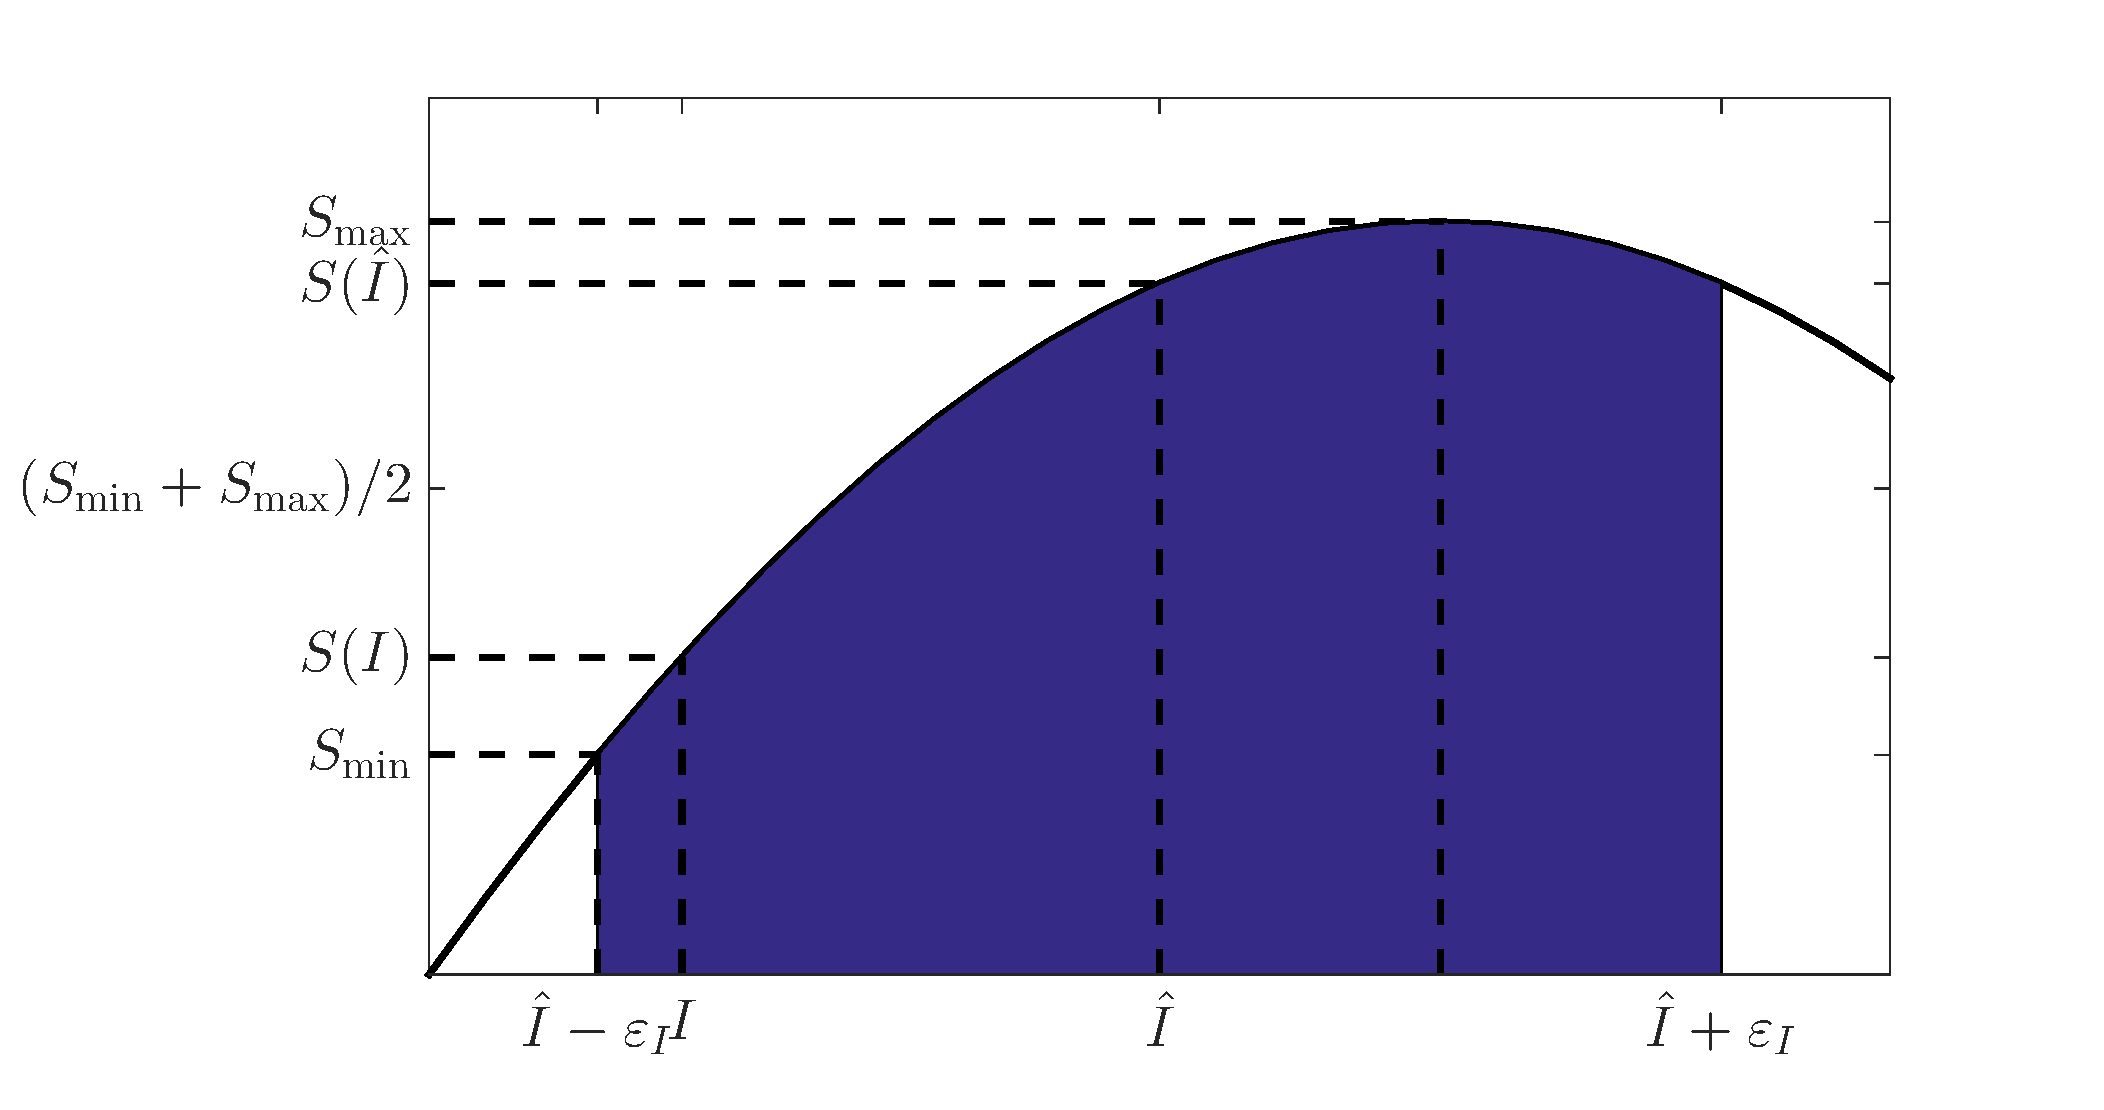
\includegraphics[width=0.75\textwidth]{scheme_S.eps}
% figure caption is below the figure
%\caption{Estimator property.}
%\label{fig:1}       % Give a unique label
%\end{figure*} 

Under the assumption that each integrand of $\vI$ is in $\cc$, these new estimators satisfy: \[ \underline{S}_u\in \left[ \widehat{\underline{S}}_u - \varepsilon_{\underline{S}_u}, \widehat{\underline{S}}_u + \varepsilon_{\underline{S}_u} \right], \qquad \overline{S}_u\in \left[ \widehat{\overline{S}}_u - \varepsilon_{\overline{S}_u}, \widehat{\overline{S}}_u + \varepsilon_{\overline{S}_u} \right] .\]
For the rest of the paper, we will consider $\widehat{\underline{S}}_u$ and $\widehat{\overline{S}}_u$   as defined in formulas (\ref{formula_undersu}) and (\ref{formula_oversu}).

\section{Sequential estimation procedure}
\label{sec:4}
The sequential estimation procedure we propose combines the error bounds $\varepsilon_{\underline{S}_u}$ and $\varepsilon_{\overline{S}_u}$ presented in the previous section with either one of the two estimation strategies of section \ref{sec:2.2}: Saltelli's strategy and the replication procedure. 

We start by detailing our procedure in the form of an algorithm. Then, we discuss a possible improvement by considering a new estimator recently introduced in \cite{Owen} for the estimation of first-order indices.

\subsection{Sequential algorithm and its cost}
\label{sec:4.1}

Algorithm \ref{recursive.algorithm} summarizes the main steps of our sequential procedure. First, one must fix the tolerance $\epsilon >0$ for the Sobol' estimates. Then, we set $m=m_0$ and construct the two designs $\mathcal{P}_{m}=\{\vx_i\}_{i=0}^{2^{m}-1}$ and $\mathcal{P}'_{m}=\{\vx'_i\}_{i=0}^{2^{m}-1}$ accordingly to the multiplicative approach detailed in \cite{GJAHMP}.  Step $5$ corresponds to the recursive scheme of this approach. The choice of $m_0$ must be large enough to ensure that each integrand of $\vI$ (Section \ref{sec:3.2}) is in $\cc$ (see  (\ref{conecond})).

With this construction, $\mathcal{P}_{m}$ and $\mathcal{P}'_{m}$ correspond to the first $2^{m}$ points of two independent Sobol' sequences. Furthermore, they possess the structure of two replicated designs of order $1$ (Definition \ref{rep.designs}).
\bigskip

$\mathcal{P}_{m}$ and $\mathcal{P}'_{m}$ can be used with Saltelli's strategy to estimate all first-order indices and total effect Sobol' indices. This option is referred as Variant $A$ in Algorithm \ref{recursive.algorithm}.

Alternatively, $\mathcal{P}_{m}$ and $\mathcal{P}'_{m}$ can be used with the replication procedure to estimate all first-order Sobol' indices. This option is referred as Variant $B$ in Algorithm \ref{recursive.algorithm}. 

In both cases we test if the respective error bounds $\varepsilon_{\underline{S}_u}$ and $\varepsilon_{\overline{S}_u}$ are lower than the tolerance $\epsilon$. For Variant $A$ the stopping criterion writes: $ \forall u \in \mathcal{D}, \varepsilon_{\underline{S}_u} \leq \epsilon \text{ and } \varepsilon_{\overline{S}_u} \leq \epsilon$,
for Variant $B$ it writes:
$ \forall u \in \mathcal{D}, \varepsilon_{\underline{S}_u} \leq \epsilon.$ 

If the stopping criterion is satisfied, the algorithm stops and Sobol' estimates are returned. Otherwise, $m$ is incremented by one to perform a new estimation. 
\begin{algorithm}[!ht]
\caption{Sequential estimation of Sobol' indices}
\begin{algorithmic}[1]
\vspace*{0.2cm}
\State choose $\epsilon >0$
\State set: $m \leftarrow m_0$
\State $bool \leftarrow false$
\While {$! bool$}
\State $\mathcal{P}_m \leftarrow \mathcal{P}_{m-1} \cup B_m$

\hspace*{-0.3cm} $\mathcal{P}'_m \leftarrow \mathcal{P}'_{m-1} \cup {B'}_m$
\For {$u =1,\dots,d$}
\If {Variant $A$}
\State estimate $\widehat{\underline{S}}_u$ and $\widehat{\ov{$S$}}_u$ with formulas (\ref{formula_undersu}) and (\ref{formula_oversu}) and Saltelli's strategy
\State $bool_u \leftarrow \varepsilon_{\underline{S}_u} \leq \epsilon \ \& \ \varepsilon_{\overline{S}_u} \leq \epsilon$
\EndIf
\If {Variant $B$}
\State estimate $\widehat{\underline{S}}_u$ with formula (\ref{formula_undersu}) and the replication procedure
\State $bool_u \leftarrow \varepsilon_{\underline{S}_u} \leq \epsilon$
\EndIf
\EndFor
\State $bool \leftarrow \forall u: \ bool_u$
\State $m \leftarrow m + 1$
\EndWhile
\State return the Sobol' estimates.
\end{algorithmic}
\label{recursive.algorithm}
\end{algorithm}
\bigskip

The cost of our algorithm varies whether Variant $A$ or Variant $B$ is selected. To discuss this cost we note by $m^\star$ the ending iteration. If Variant $A$ is selected, the cost of our algorithm writes:
\[\sum \limits_{u \in \mathcal{D}} 2^{m_u} + 2 \times 2^{m^{\star}}, \qquad m^\star= \max \limits_{u \in \mathcal{D}} \ m_u,\]
where: 
\begin{itemize}
\item[$\bullet$] $2^{m_u}$ is the number of evaluations $f\left(\vx_{i,u}:{\vx'}_{i,-u}\right)$ used to estimate both the first-order index $\underline{S}_u$ and the total effect index $\overline{S}_u$,
\item[$\bullet$] $2 \times 2^{m^{\star}}$ is the number of evaluations $f\left(\vx_{i}\right)$ and $f\left({\vx'}_{i}\right)$ used in the estimation of each first-order and total effect indices.
\end{itemize}
If all $m_u$ are equal, the cost of Variant $A$ becomes $2^{m^\star}(d+2)$ and we recover the cost specified in Theorem \ref{saltelli.theorem} with $n=2^{m^\star}$.

If Variant $B$ is selected the cost of our algorithm equals $2 \times 2^{m^{\star}}$. This cost corresponds to the one of the replication procedure claimed in the introduction, where $2n=2\times 2^{m^{\star}}$ independent of $d$.

\subsection{Improvement}
\label{sec:4.2}

We focus on the use of a new estimator to evaluate small first-order Sobol' indices in Variant $A$. This estimator has recently been introduced by Owen in \cite{Owen} and is called ``Correlation 2". Owen discussed and highlighted the efficiency of ``Correlation 2" when estimating small first-order indices. Our aim is to show that using ``Correlation 2" in Variant $A$ may reduce the total number of model evaluations. Its formula writes as follows:
\begin{equation*}
\widehat{\underline{\tau}_u^2} = \frac{1}{n} \sum \limits_{i=0}^{n-1} (f(\vx_i)-f({\vz}_{i,u}:{\vx}_{i,-u}))(f(\vx_{i,u}:{\vx'}_{i,-u})-f({\vx'}_i)),
\end{equation*}
where $(\vx_i,{\vx'}_i, \vz_i) \iid [0,1)^{3d}$. It uses an extra set of $n$ model evaluations to estimate $\underline{\tau}_u^2$.
\bigskip

We discuss below the potential improvement brought by using ``Correlation 2" in Variant $A$. The idea is to replace the current estimator (\ref{first.order.est}) by  ``Correlation 2" for each small first-order indices. 

Assume that the number of small first-order indices is known and equals $\gamma$. We denote by $u_1,\dots,u_{\gamma}$ the indices of the corresponding inputs and $\Gamma = \{1,\dots,\gamma\}$. The cost of Variant $A$ including ``Correlation 2" writes: 
\begin{equation}
\sum \limits_{j \in \Gamma} 2^{m''_{u_j}} + \sum \limits_{j \in \Gamma} 2^{m'_{u_j}} + \sum \limits_{j \in \mathcal{D}\setminus{\Gamma}} 2^{m_{u_j}} + 2 \times 2^{m^\star},
\label{cost.improvement}
\end{equation}
where $m'_{u_j}\leq m^{\star}$, $\ m_{u_j} \leq m^{\star}$, and: 
\begin{itemize}
\item[$\bullet$] for $j\in \Gamma$, $2^{m''_{u_j}}$ is the number of evaluations \\ $f\left(\vz_{i,u_j}:\vx_{i,-u_j}\right)$ to estimate $\underline{S}_{u_j}$,
\item[$\bullet$] for $j\in \Gamma$, $2^{m'_{u_j}}$ is the number of evaluations \\ $f\left(\vx_{i,u_j}:{\vx'}_{i,-u_j}\right)$ to estimate both $\underline{S}_{u_j}$ and  $\overline{S}_{u_j}$,
\item[$\bullet$] likewise, for $j\in \mathcal{D}\setminus{\Gamma}$, $ 2^{m_{u_j}}$ is the number of evaluations $f\left(\vx_{i,u_j}:{\vx'}_{i,-u_j}\right)$ to estimate both $\underline{S}_{u_j}$ and  $\overline{S}_{u_j}$,
\item[$\bullet$] $2 \times 2^{m^{\star}}$ is the number of evaluations $f\left(\vx_{i}\right)$ and $f\left({\vx'}_{i}\right)$ used in the estimation of each first-order and total effect index.
\end{itemize}
Recall that the cost of Variant $A$ without  ``Correlation 2" writes:
\begin{equation}
\sum \limits_{j \in \Gamma} 2^{m_{u_j}} + \sum \limits_{j \in \mathcal{D}\setminus{\Gamma}} 2^{m_{u_j}} + 2 \times 2^{m^{\star}}, \qquad m_{u_j} \leq m^{\star}.
\label{cost.non.improvement}
\end{equation}
The difference between costs (\ref{cost.improvement}) and (\ref{cost.non.improvement}) equals:
\begin{equation}
 \sum \limits_{j \in \Gamma} 2^{m_{u_j}} \left(2^{m''_{u_j}-m_{u_j}}  + 2^{m'_{u_j}-m_{u_j}} - 1 \right) = \sum \limits_{j \in \Gamma} c_j.
\label{cost.comparison}
\end{equation}
Hence, the sign of this difference indicates whether or not using ``Correlation 2" brings an improvement to Variant $A$. We distinguish two cases :
\begin{itemize}
\item[1)] for $j \in \Gamma$, the total effect index $\ov{$S$}_{u_j}$ requires as much or more evaluations than the first-order index $\underline{S}_{u_j}$. Since the total effect estimator is the same, as a consequence we have $m'_{u_j}=m_{u_j}$ and $c_j >0$.
\item[2)] for $j \in \Gamma$, the total effect index $\ov{$S$}_{u_j}$ requires less evaluations than the first-order index $\underline{S}_{u_j}$. In this case, if both $m''_{u_j} < m_{u_j}$ and $m'_{u_j} < m_{u_j}$ then $c_j \leq 0$.  
\end{itemize}
Overall we expect to observe case $2)$ more often than case $1)$. Indeed, the numerator of $\underline{S}_u$ requires to estimate $2d-1$ dimensional integrals against only $d+1$ dimensional integrals for the numerator of $\ov{$S$}_u$. Hence, it seems reasonable to expect that it will take less points to estimate $\ov{$S$}_u$ than $\underline{S}_u$. 

Furthermore, in case $2)$, we expect the two conditions $m''_{u_j} < m_{u_j}$ and $m'_{u_j} < m_{u_j}$ to always hold as ``Correlation 2" is shown 
to perform better for small first-order indices. To support this discussion, illustrations of the use of ``Correlation 2" are presented in Section \ref{sec:5}. 

In practice, one does not know which are the small Sobol' indices. To overcome this issue, we propose the following alternative for Variant $A$. If at the end of the first iteration, the estimate $\widehat{\underline{S}}_u$, $u \in \mathcal{D}$, is smaller than a threshold, then at the next iteration estimator (\ref{first.order.est}) is switched for ``Correlation 2" and a third Sobol' sequence $\mathcal{P''}_{m}=\{\vz_i\}_{i=0}^{2^m-1}$ is constructed to obtain the corresponding evaluations $f({\vz}_{i,u}:{\vx}_{i,-u})$.

\section{Applications}
\label{sec:5}
\subsection{Real case model}
\label{sec:5.1}
%The Brownian motion is widely used in many applications. Thus, the following example might be interesting to understand what Sobol' indices can explain in some of these applications. For instance, if we want to estimate the expected value of the maximum of a discretized Brownian motion whose covariance matrix is $\Sigma$, our goal is to estimate
%\begin{align*}
%\mathbb{E} \left[\max(\vect{B}_t)\right] &= \int_{\mathbb{R}^d} \max(\vect{B}_t) \frac{{\rm e}^{\vect{B}_t^T\Sigma^{-1}\vect{B}_t}}{(2\pi)^{d/2}|\Sigma|^{1/2}}\,d\vect{B}_t \\
%&= \int_{[0,1]^d} \max(f_{\rm Chol}(\vx)) \,d\vx \\
%&= \int_{[0,1]^d} \max(f_{\rm PCA}(\vx)) \,d\vx.
%\end{align*}
%The last two equalities are obtained through two different subsitutions corresponding to the \textit{Cholesky} construction of the Brownian motion, and the \textit{PCA} construction. For instance, if we take 10 dimensions and $t_i=i/10$, using the Cholesky construction $S_{1} = 24\%$, $S_{2} = 16\%$, $S_{3} = 13\%$, $S_{4} = 10\%$, and $\overline{S}_{1}=24\%$, $\overline{S}_{2}=18\%$, $\overline{S}_{3}=15\%$, $\overline{S}_{4} = 13\%$. However, using the PCA construction, $S_{1} = 89\%$, $S_{2} = 2\%$, $S_{3} = 1\%$, $S_{4} = 0\%$, and $\overline{S}_{1}=94\%$, $\overline{S}_{2}=7\%$, $\overline{S}_{3}=3\%$, $\overline{S}_{4} = 2\%$. This shows that the PCA construction will be better to estimate the above expectation using quasi-Monte Carlo methods since it has a lower effective dimensionality.
%
%For those who were curious about the actual value of $\mathbb{E} \left[\max(\vect{B}_t)\right]$, it is approximately 0.5935. Nevertheless, the Brownian Motion is a continuous time process. Thus, in order to estimate the expected value on a continuous time Browninan motion, one could either use a multilevel method, or a multivariate decomposition method to estimate this infinite dimensional integral.

\subsection{Classical test functions}
\label{sec:5.2}

\begin{acknowledgements}
This work is supported by the CITiES project funded by the Agence Nationale de la Recherche (grant ANR-12-\newline MONU-0020) and by the United States National Science Foundation (grant DMS-1522687).

The authors thank Fred J. Hickernell and Cl\'ementine Prieur for initiating this collaborative work and Elise Arnaud for her proofreading. The authors are grateful to Stephen Joe, Frances Y. Kuo and Art B. Owen for their helpful answers and suggestions.   
\end{acknowledgements}

% BibTeX users please use one of
%\bibliographystyle{spbasic}      % basic style, author-year citations
%\bibliographystyle{spmpsci}      % mathematics and physical sciences
%\bibliographystyle{spphys}       % APS-like style for physics
%\bibliography{}   % name your BibTeX data base

% Non-BibTeX users please use
\begin{thebibliography}{99}
%
% and use \bibitem to create references. Consult the Instructions
% for authors for reference list style.
%
\bibitem{Gilquin.rec}
Gilquin, L., Arnaud, E., Monod, H., Prieur, C.: Recursive estimation procedure of Sobol' indices based on replicated designs, preprint available at \url{https://hal.inria.fr/hal-01291769}, (2016).
\bibitem{GJAHMP}
Gilquin, L., Jim\'enez Rugama, Ll.A., Arnaud, E., Hickernell, F.J., Monod, H., Prieur, C.: Iterative construction of replicated designs based on Sobol' sequences, preprint available at \url{https://hal.inria.fr/hal-01349444} (2016)
\bibitem{HicJim}
Hickernell, F.J., Jim\'enez Rugama, Ll.A.: Reliable Adaptative Cubature Using Digital Sequences: Monte Carlo and Quasi-Monte Carlo Methods, vol. 163, 367-383 (2016)
\bibitem{Hoeffding}
Hoeffding, W.F.: A class of statistics with asymptotically normal distribution, Ann. Math. Stat. \textbf{19}(3), 293-325 (1948)
%\bibitem{Janon}
%Janon, A., Klein, T., Lagnoux A., Nodet, M., Prieur C.: Asymptotic normality and efficiency of two {S}obol' index estimators, ESAIM Probab. Stat. \textbf{18}, 342-364 (2014)
\bibitem{Lemieuxbook}
Lemieux,C.: Monte Carlo and Quasi-Monte Carlo Sampling, Springer, New-York (2009)
\bibitem{Mara}
Mara, T.A., Rakoto Joseph, 0.: Comparison of some efficient methods to evaluate the main effect of computer model factors, J. Statist. Comput. Simulation \textbf{78}(2), 167-178 (2008)
\bibitem{McKay}
McKay, M.D.: Evaluating prediction uncertainty, Los Alamos National Laboratory Report NUREG/CR- 6311, LA-12915-MS. (1995)
\bibitem{Niederreiter} 
Niederreiter, H.: Random Number Generation and Quasi-Monte Carlo Methods: CBMS-NSF Regional Conference Series in Applied Math., vol. 63, SIAM, Philadelphia (1992)
\bibitem{Owen}
Owen, A.B.: Better estimation of small Sobol' sensitivity indices, ACM Trans. Model. Comput. Simul. \textbf{23}(2), :11 (2013)
\bibitem{Saltelli}
Saltelli, A.: Making best use of models evaluations to compute sensitivity indices, Comput. Phys. Commun. \textbf{145}(2), 280-297 (2002)
\bibitem{Sobol'seq}
Sobol', I.M.: On the distribution of points in a cube and the approximate evaluation of integrals, USSR Comput. Math. Math. Phys. \textbf{7}(4), 86-112 (1967)
\bibitem{Sobol'}
Sobol', I.M.: Sensitivity indices for nonlinear mathematical models, Mathematical Modeling and Computational Experiment \textbf{1}, 407-414 (1993)
\bibitem{Tissot}
Tissot, J.Y., Prieur, C.: A randomized Orthogonal Array-based procedure for the estimation of first- and second-order Sobol' indices, J. Statist. Comput. Simulation \textbf{85}(7), 1358-1381 (2015)
\bibitem{Tong}
Tong C.: Self-validated variance-based methods for sensitivity analysis of model outputs, Reliab. Eng. Syst. Saf. \textbf{95}(3), 301-309 (2010)

\end{thebibliography}
\end{document}
